\documentclass[a4paper,12pt]{article}

\setlength{\parskip}{\baselineskip} % Spacing between paragraphs
\setlength{\parindent}{0pt} % Don't indent new paragraphs

\usepackage{tikz}
\tikzset{
	treenode/.style = {align=center, inner sep=0pt, text centered,  font=\small},
	explored/.style = {treenode, circle, black, draw=black,  text width=1.2em},
	hid/.style = {treenode, circle, lightgray, dashed},
	pruned/.style = {treenode, circle, lightgray, dashed, draw=black, font=\sffamily\bfseries, text width=1.2em},
	expr/.style = {treenode, draw=black},
	dead/.style = {treenode, draw=black}
}

% Floating picture next to each other
\usepackage{floatrow}
\usepackage{subfig}
\floatsetup[figure]{style=plain,subcapbesideposition=center}

\usepackage{standalone}

% Title etc...
\title{COMP9814:\\Assignment 2 - Heuristics and Search}

\author{Alexander Whillas\\
\small School of Computer Science and Engineering\\[-0.8ex]
\small University of New South Wales\\[-0.8ex]
\small Sydney, Australia\\
\small \texttt{z3446737@student.unsw.edu.au}
}
\date{May 5, 2013}

\begin{document}
\maketitle
\newpage


\section*{Question 1 - Graph Paper Grand Prix}

(a) Where $k = 0$ the following is the output from $M(n, 0)$ for $1 < n < 21$:

\begin{center}
\begin{tabular}{llccccccc}
\hline
$n$ & optimal sequence & + & o & - & t & $M(n,0)$ & $2s + 1$ & $2s + 2$\\
\hline
0  &  & 0 & 0 & 0 & 0 & 0 & 1 & 2\\
1  & + - & 1 & 0 & 1 & 2 & 2 & 3 & 4\\
2  & + o - & 1 & 1 & 1 & 3 & 3 & 3 & 4\\
3  & + o o - & 1 & 2 & 1 & 4 & 4 & 3 & 4\\
4  & + + - - & 2 & 0 & 2 & 4 & 4 & 5 & 6\\
5  & + + - o - & 2 & 1 & 2 & 5 & 5 & 5 & 6\\
6  & + + o - - & 2 & 1 & 2 & 5 & 5 & 5 & 6\\
7  & + + o - o - & 2 & 2 & 2 & 6 & 6 & 5 & 6\\
8  & + + o o - - & 2 & 2 & 2 & 6 & 6 & 5 & 6\\
9  & + + + - - - & 3 & 0 & 3 & 6 & 6 & 7 & 8\\
10 & + + + - - o - & 3 & 1 & 3 & 7 & 7 & 7 & 8\\
11 & + + + - o - - & 3 & 1 & 3 & 7 & 7 & 7 & 8\\
12 & + + + o - - - & 3 & 1 & 3 & 7 & 7 & 7 & 8\\
13 & + + + o - - o - & 3 & 2 & 3 & 8 & 8 & 7 & 8\\
14 & + + + o - o - - & 3 & 2 & 3 & 8 & 8 & 7 & 8\\
15 & + + + o o - - - & 3 & 2 & 3 & 8 & 8 & 7 & 8\\
16 & + + + + - - - - & 4 & 0 & 4 & 8 & 8 & 9 & 10\\
17 & + + + + - - - o - & 4 & 1 & 4 & 9 & 9 & 9 & 10\\
18 & + + + + - - o - - & 4 & 1 & 4 & 9 & 9 & 9 & 10\\
19 & + + + + - o - - - & 4 & 1 & 4 & 9 & 9 & 9 & 10\\
20 & + + + + o - - - - & 4 & 1 & 4 & 9 & 9 & 9 & 10\\
21 & + + + + o - - - o - & 4 & 2 & 4 & 10 & 10 & 9 & 10\\
\hline
\end{tabular}
\end{center}

\medskip


(b) I the above table the $t$ column is the length of the optimal sequence and $M(n,0)$  was calculated with the following formula
\begin{equation}
	M(n, 0) = \left\lceil 2\sqrt{n} \right\rceil
\end{equation}
We can see that $t$ agrees with the $M(n, 0)$ all of the time. If we assume the following identity

\begin{equation}
\left\lceil 2\sqrt{n} \right\rceil = \left\{
	\begin{array}{lrcl}
		2s + 1\ \mbox{if} &	  s^2 & <\ n & \leq s(s + 1) \\
		2s + 2\ \mbox{if} & s(s + 1) & <\ n & \leq (s + 1)^2
	\end{array} \right.
\end{equation}

where $s$ is the maximum speed (the number of `$+$'s, $+$ column),
then the identity holds for $s(s + 1)$ when there is one rest (i.e. a `$o$')
and $s(s + 1)$ when there are two rests.

The only exception to this is when $n$ is 2, 4, 9 or 16 i.e. $n$ is a perfect square. Then the value from the identity is too high by 1 since $s^2 = n$.\medskip


(c) If $k \geq 0$ then we are starting with some $k$ at $S$ and if $n \geq  k (K - 1)$ then we stop at or before $G$ (distance of $n$). So if we assume this roughly the second half of $M(n,0)$ i.e. the deceleration time, then equation (1) becomes the total distance $x$ less the time it took to accelerate to velocity $k$ that is

\begin{equation}
	M(x, 0) = \left\lceil 2\sqrt{x} \right\rceil - k
\end{equation}
where $x$ is the total distance to accelerate to velocity $k$ given by the Gaussian summation formula

\begin{equation}
	\frac{k(k + 1)}{2}
\end{equation}
and $n$. Substituting these into (3) for $x$ gives

\begin{equation}
	M(n, k) = \left\lceil 2\sqrt{n + \frac{k(k + 1)}{2}} \ \right\rceil - k
\end{equation}


(d) Taking the same approach as (c) except $n <  k (K - 1)$ thus we overshoot the goal $G$ and have to reverse to it. So $x > n$ and the total distance is now
\begin{equation}
	\begin{array}{rlclcl}
	M(n, k) = & total\ overshoot\ time & + & reverse\ time & - & acceleration\ time \\
	M(n, k) = & \left\lceil 2\sqrt{\frac{k(k + 1)}{2} + \frac{k(k - 1)}{2}} \ \right\rceil & + & \left\lceil 2\sqrt{\frac{k(k - 1)}{2} - n} \
\right\rceil & - & k
	\end{array}
\end{equation}
the first term simplifies down to $2k$ (which makes sense) leaving us with
\begin{equation}
	M(n, k) = \left\lceil 2\sqrt{\frac{k(k - 1)}{2} - n} \ \right\rceil + k
\end{equation}


(e) Extrapolating the work above from 1-dimensional to 2-dimensional for the GPGP game we get
\begin{equation}
	h(r,c,u,v,r_G,c_G) = max(M(r_G - r, u), M(c_G - c, v))
\end{equation}
where M is given by the equation (5) above.

This an \emph{admissible} heuristic as it only takes one dimension, the longest, into account thus under estimates the cars performance. Even if it were to take the hypotenuse distance this would, in most cases, be in accurate as the GPGP is not normally a straight line.

\section*{Question 2 - Game Trees and Pruning}


\subsection*{Part (a)}

\begin{figure}[!h]
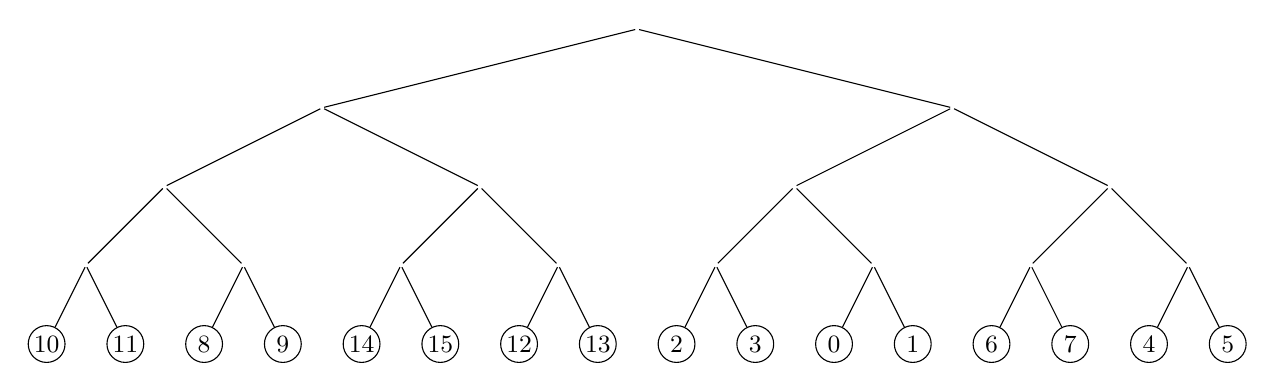
\begin{tikzpicture}[
	level/.style={level distance=1cm},
 	level 1/.style={sibling distance = 8cm},
 	level 2/.style={sibling distance = 4cm},
 	level 3/.style={sibling distance = 2cm},
 	level 4/.style={sibling distance = 1cm}
]
\node [treenode] {}
child{ node [treenode] {}
	child{ node [treenode] {}
		child{ node [treenode] {}
			child{ node [explored] {10}}
			child{ node [explored] {11}}
		}
		child{ node [treenode] {}
			child{ node [explored] {8}}
			child{ node [explored] {9}}
		}
	}
	child{ node [treenode] {}
		child{ node [treenode] {}
			child{ node [explored] {14}}
			child{ node [explored] {15}}
		}
		child{ node [treenode] {}
			child{ node [explored] {12}}
			child{ node [explored] {13}}
		}
	}
}
child{ node [treenode] {}
	child{ node [treenode] {}
		child{ node [treenode] {}
			child{ node [explored] {2}}
			child{ node [explored] {3}}
		}
		child{ node [treenode] {}
			child{ node [explored] {0}}
			child{ node [explored] {1}}
		}
	}
	child{ node [treenode] {}
		child{ node [treenode] {}
			child{ node [explored] {6}}
			child{ node [explored] {7}}
		}
		child{ node [treenode] {}
			child{ node [explored] {4}}
			child{ node [explored] {5}}
		}
	}
}
;
\end{tikzpicture}
\caption{}
\end{figure}

\newpage

\subsection*{Part (b)}

\begin{figure}[!htbp]% h=here allowed, t=top, b=bottom, p=on a float-page
	\sidesubfloat[]{%
		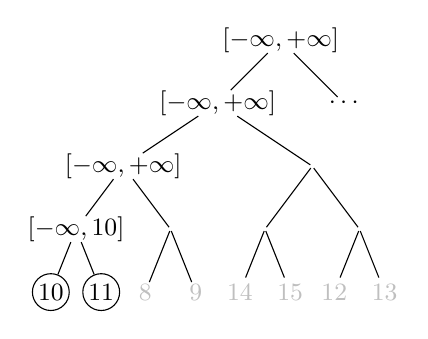
\begin{tikzpicture}[scale=0.8,
			level/.style={level distance=1cm},
		 	level 1/.style={sibling distance = 2cm},
		 	level 2/.style={sibling distance = 3cm},
		 	level 3/.style={sibling distance = 1.5cm},
		 	level 4/.style={sibling distance = 0.8cm}
		]
		\node [treenode] {[$-\infty, +\infty$]}
		child{ node [treenode] {[$-\infty, +\infty$]}
			child{ node [treenode] {[$-\infty, +\infty$]}
				child{ node [treenode] {[$-\infty, 10$]}
					child{ node [explored] {10}}
					child{ node [explored] {11}}
				}
				child{ node [treenode] {}
					child{ node [hid] {8}}
					child{ node [hid] {9}}
				}
			}
			child{ node [treenode] {}
				child{ node [treenode] {}
					child{ node [hid] {14}}
					child{ node [hid] {15}}
				}
				child{ node [treenode] {}
					child{ node [hid] {12}}
					child{ node [hid] {13}}
				}
			}
		}
		child{ node [treenode] {$\cdots$} }
		;
		\end{tikzpicture}
	}
	\qquad%
	\sidesubfloat[]{%
		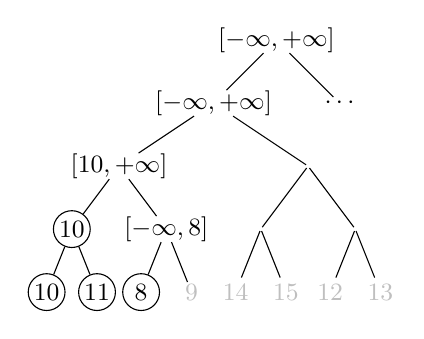
\begin{tikzpicture}[scale=0.8,
			level/.style={level distance=1cm},
		 	level 1/.style={sibling distance = 2cm},
		 	level 2/.style={sibling distance = 3cm},
		 	level 3/.style={sibling distance = 1.5cm},
		 	level 4/.style={sibling distance = 0.8cm}
		]
		\node [treenode] {[$-\infty,+\infty$]}
		child{ node [treenode] {[$-\infty, +\infty$]}
			child{ node [treenode] {[$10, +\infty$]}
				child{ node [explored] {10}
					child{ node [explored] {10}}
					child{ node [explored] {11}}
				}
				child{ node [treenode] {[$-\infty, 8$]}
					child{ node [explored] {8}}
					child{ node [hid] {9}}
				}
			}
			child{ node [treenode] {}
				child{ node [treenode] {}
					child{ node [hid] {14}}
					child{ node [hid] {15}}
				}
				child{ node [treenode] {}
					child{ node [hid] {12}}
					child{ node [hid] {13}}
				}
			}
		}
		child{ node [treenode] {$\cdots$} }
		;
		\end{tikzpicture}
	}
	\qquad%
	\bigbreak%
	\sidesubfloat[]{%
		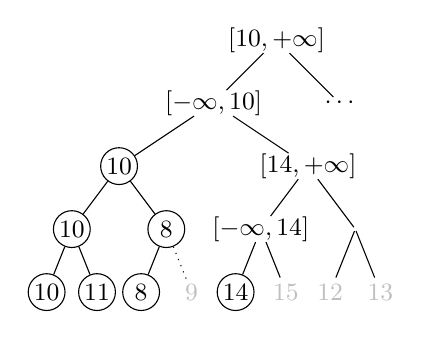
\begin{tikzpicture}[scale=0.8,
			level/.style={level distance=1cm},
		 	level 1/.style={sibling distance = 2cm},
		 	level 2/.style={sibling distance = 3cm},
		 	level 3/.style={sibling distance = 1.5cm},
		 	level 4/.style={sibling distance = 0.8cm}
		]
		\node [treenode] {[$10, +\infty$]}
		child{ node [treenode] {[$-\infty, 10$]}
			child{ node [explored] {10}
				child{ node [explored] {10}
					child{ node [explored] {10}}
					child{ node [explored] {11}}
				}
				child{ node [explored] {8}
					child{ node [explored] {8}}
					child[dotted]{ node [hid] {9}}
				}
			}
			child{ node [treenode] {[$14, +\infty$]}
				child{ node [treenode] {[$-\infty, 14$]}
					child{ node [explored] {14}}
					child{ node [hid] {15}}
				}
				child{ node [treenode] {}
					child{ node [hid] {12}}
					child{ node [hid] {13}}
				}
			}
		}
		child{ node [treenode] {$\cdots$} }
		;
		\end{tikzpicture}
	}
	\qquad%
	\sidesubfloat[]{%
		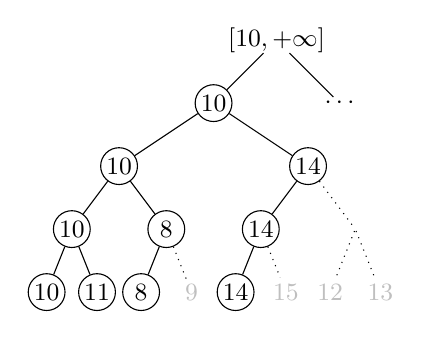
\begin{tikzpicture}[scale=0.8,
			level/.style={level distance=1cm},
		 	level 1/.style={sibling distance = 2cm},
		 	level 2/.style={sibling distance = 3cm},
		 	level 3/.style={sibling distance = 1.5cm},
		 	level 4/.style={sibling distance = 0.8cm}
		]
		\node [treenode] {[$10, +\infty$]}
		child{ node [explored] {10}
			child{ node [explored] {10}
				child{ node [explored] {10}
					child{ node [explored] {10}}
					child{ node [explored] {11}}
				}
				child{ node [explored] {8}
					child{ node [explored] {8}}
					child[dotted]{ node [hid] {9}}
				}
			}
			child{ node [explored] {14}
				child{ node [explored] {14}
					child{ node [explored] {14}}
					child[dotted]{ node [hid] {15}}
				}
				child[dotted]{ node [treenode] {}
					child{ node [hid] {12}}
					child{ node [hid] {13}}
				}
			}
		}
		child{ node [treenode] {$\cdots$} }
		;
		\end{tikzpicture}
	}
	\qquad%
	\bigbreak%
	\sidesubfloat[]{%
		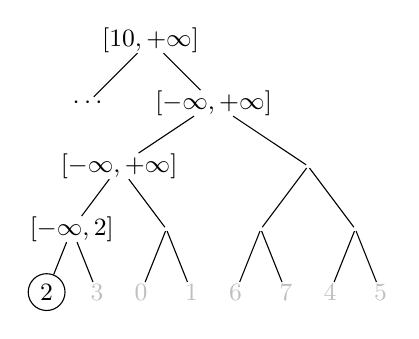
\begin{tikzpicture}[scale=0.8,
			level/.style={level distance=1cm},
		 	level 1/.style={sibling distance = 2cm},
		 	level 2/.style={sibling distance = 3cm},
		 	level 3/.style={sibling distance = 1.5cm},
		 	level 4/.style={sibling distance = 0.8cm}
		]
		\node [treenode] {[$10, +\infty$]}
		child{ node [treenode] {$\cdots$} }
		child{ node [treenode] {$[-\infty, +\infty]$}
			child{ node [treenode] {$[-\infty, +\infty]$}
				child{ node [treenode] {$[-\infty, 2]$}
					child{ node [explored] {2}}
					child{ node [hid] {3}}
				}
				child{ node [treenode] {}
					child{ node [hid] {0}}
					child{ node [hid] {1}}
				}
			}
			child{ node [treenode] {}
				child{ node [treenode] {}
					child{ node [hid] {6}}
					child{ node [hid] {7}}
				}
				child{ node [treenode] {}
					child{ node [hid] {4}}
					child{ node [hid] {5}}
				}
			}
		}
		;
		\end{tikzpicture}
	}
	\qquad%
	\sidesubfloat[]{%
		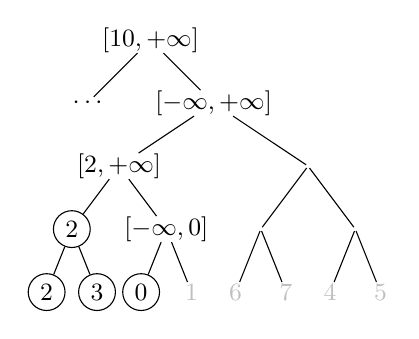
\begin{tikzpicture}[scale=0.8,
			level/.style={level distance=1cm},
		 	level 1/.style={sibling distance = 2cm},
		 	level 2/.style={sibling distance = 3cm},
		 	level 3/.style={sibling distance = 1.5cm},
		 	level 4/.style={sibling distance = 0.8cm}
		]
		\node [treenode] {[$10, +\infty$]}
		child{ node [treenode] {$\cdots$} }
		child{ node [treenode] {$[-\infty, +\infty]$}
			child{ node [treenode] {$[2, +\infty]$}
				child{ node [explored] {2}
					child{ node [explored] {2}}
					child{ node [explored] {3}}
				}
				child{ node [treenode] {$[-\infty, 0]$}
					child{ node [explored] {0}}
					child{ node [hid] {1}}
				}
			}
			child{ node [treenode] {}
				child{ node [treenode] {}
					child{ node [hid] {6}}
					child{ node [hid] {7}}
				}
				child{ node [treenode] {}
					child{ node [hid] {4}}
					child{ node [hid] {5}}
				}
			}
		}
		;
		\end{tikzpicture}
	}
	\qquad%
	\bigbreak%
	\sidesubfloat[]{%
		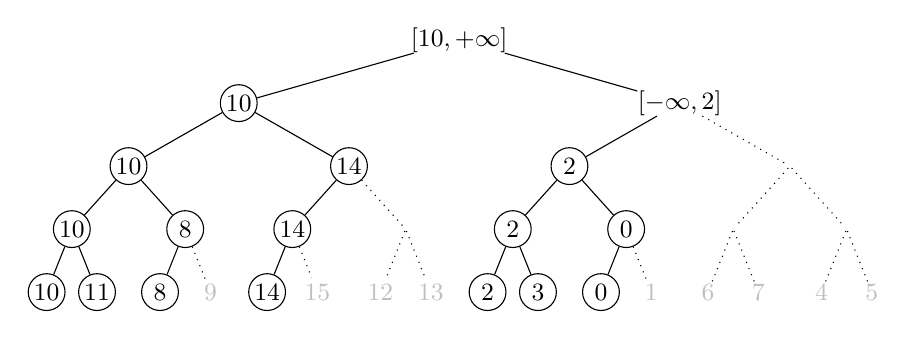
\begin{tikzpicture}[scale=0.8,
			level/.style={level distance=1cm},
		 	level 1/.style={sibling distance = 7cm},
		 	level 2/.style={sibling distance = 3.5cm},
		 	level 3/.style={sibling distance = 1.8cm},
		 	level 4/.style={sibling distance = 0.8cm}
		]
		\node [treenode] {[$10, +\infty$]}
		child{ node [explored] {10}
			child{ node [explored] {10}
				child{ node [explored] {10}
					child{ node [explored] {10}}
					child{ node [explored] {11}}
				}
				child{ node [explored] {8}
					child{ node [explored] {8}}
					child[dotted]{ node [hid] {9}}
				}
			}
			child{ node [explored] {14}
				child{ node [explored] {14}
					child{ node [explored] {14}}
					child[dotted]{ node [hid] {15}}
				}
				child[dotted]{ node [treenode] {}
					child{ node [hid] {12}}
					child{ node [hid] {13}}
				}
			}
		}
		child{ node [treenode] {$[-\infty, 2]$}
			child{ node [explored] {2}
				child{ node [explored] {2}
					child{ node [explored] {2}}
					child{ node [explored] {3}}
				}
				child{ node [explored] {0}
					child{ node [explored] {0}}
					child[dotted]{ node [hid] {1}}
				}
			}
			child[dotted]{ node [treenode] {}
				child{ node [treenode] {}
					child{ node [hid] {6}}
					child{ node [hid] {7}}
				}
				child{ node [treenode] {}
					child{ node [hid] {4}}
					child{ node [hid] {5}}
				}
			}
		}
		;
		\end{tikzpicture}
	}
	\caption{}
\end{figure}

Figure 2 is illustrated the process of the \emph{Aplha-Beta} pruning on the tree in Part (a). Note the grey numbers are \emph{to be} explored and the dotted lines are \emph{pruned} branches of the tree. In (a), just looking at the left side of the tree, the left most branch is explored first and a 10 is discover which is better than the current $\beta$ value of $-\infty$. The leaf node 11 is then explored. (b) MIN chooses 10 and sets its parent $\alpha$ to this. The left most side of the next branch is explored to reveal an 8 which becomes the new $\beta$ of its parent MIN node. (c) the leaf node 9 gets pruned as the parent $\alpha$ (10) is greater than the child $\beta$ (8). Then leaf node 14 branch is explored. (d) since the 2nd level MIN node has $\beta = 10$ thus the 14 will never be chosen by MIN so the 15, 12 and 13 branches are pruned. (e) we switch over to the right hand side of the tree with the root nodes $\alpha$ set to 10. The 2 leaf node is explored  and its parent $\beta$ set to 2. (f) The leaf node 3 is explored and the parent is set to 2 as a result of $MIN(2, 3)$. The parent MAX has its $\alpha$ set to 2. The leaf node 0 is explored and its parent $\beta$ set to 0. (g) Since the 3rd level MAX has $\alpha = 2$ and its right child node's $beta = 2$, the leaf node 1 is pruned and the 2 propagated up the the parent MIN nodes $beta$. Since the root nodes $alpha$ (10) is greater than the MIN child's $beta$ (2), ensuring this will never be greater than 2, the root MAX will always choose the left 10 and the search terminates here.

\subsection*{Part (c): Pruning pattern}

\begin{figure}[!h]
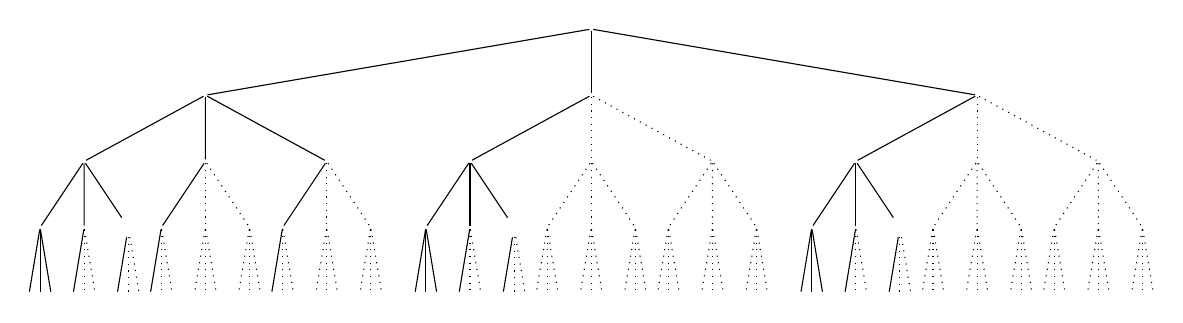
\begin{tikzpicture}[scale=0.7,
	level/.style={level distance=1.2cm},
 	level 1/.style={sibling distance = 7cm},
 	level 2/.style={sibling distance = 2.2cm},
 	level 3/.style={sibling distance = 0.8cm},
 	level 4/.style={sibling distance = 0.2cm},
]
\node [treenode] {}
child{ node [treenode] {}
	child{ node [treenode] {}
		child{ node [treenode] {}
			child{ node [treenode] {}}
			child{ node [treenode] {}}
			child{ node [treenode] {}}
		}
		child{ node [treenode] {}
			child{ node [treenode] {}}
			child[dotted]{ node [treenode] {}}
			child[dotted]{ node [treenode] {}}
		}
		child{ node{}
			child{ node [treenode] {}}
			child[dotted]{ node [treenode] {}}
			child[dotted]{ node [treenode] {}}
		}
	}
	child{ node [treenode] {}
		child{ node [treenode] {}
			child{ node [treenode] {}}
			child[dotted]{ node [treenode] {}}
			child[dotted]{ node [treenode] {}}
		}
		child[dotted]{ node [treenode] {}
			child{ node [treenode] {}}
			child{ node [treenode] {}}
			child{ node [treenode] {}}
		}
		child[dotted]{ node [treenode] {}
			child{ node [treenode] {}}
			child{ node [treenode] {}}
			child{ node [treenode] {}}
		}
	}
	child{ node [treenode] {}
		child{ node [treenode] {}
			child{ node [treenode] {}}
			child[dotted]{ node [treenode] {}}
			child[dotted]{ node [treenode] {}}
		}
		child[dotted]{ node [treenode] {}
			child{ node [treenode] {}}
			child{ node [treenode] {}}
			child{ node [treenode] {}}
		}
		child[dotted]{ node [treenode] {}
			child{ node [treenode] {}}
			child{ node [treenode] {}}
			child{ node [treenode] {}}
		}
	}
}
child{ node [treenode] {}
	child{ node [treenode] {}
		child{ node [treenode] {}
			child{ node [treenode] {}}
			child{ node [treenode] {}}
			child{ node [treenode] {}}
		}
		child{ node [treenode] {}
			child{ node [treenode] {}}
			child[dotted]{ node [treenode] {}}
			child[dotted]{ node [treenode] {}}
		}
		child{ node{}
			child{ node [treenode] {}}
			child[dotted]{ node [treenode] {}}
			child[dotted]{ node [treenode] {}}
		}
	}
	child[dotted]{ node [treenode] {}
		child{ node [treenode] {}
			child{ node [treenode] {}}
			child{ node [treenode] {}}
			child[dotted]{ node [treenode] {}}
		}
		child[dotted]{ node [treenode] {}
			child{ node [treenode] {}}
			child{ node [treenode] {}}
			child{ node [treenode] {}}
		}
		child[dotted]{ node [treenode] {}
			child{ node [treenode] {}}
			child{ node [treenode] {}}
			child{ node [treenode] {}}
		}
	}
	child[dotted]{ node [treenode] {}
		child{ node [treenode] {}
			child{ node [treenode] {}}
			child[dotted]{ node [treenode] {}}
			child[dotted]{ node [treenode] {}}
		}
		child[dotted]{ node [treenode] {}
			child{ node [treenode] {}}
			child{ node [treenode] {}}
			child{ node [treenode] {}}
		}
		child[dotted]{ node [treenode] {}
			child{ node [treenode] {}}
			child{ node [treenode] {}}
			child{ node [treenode] {}}
		}
	}
}
child{ node [treenode] {}
	child{ node [treenode] {}
		child{ node [treenode] {}
			child{ node [treenode] {}}
			child{ node [treenode] {}}
			child{ node [treenode] {}}
		}
		child{ node [treenode] {}
			child{ node [treenode] {}}
			child[dotted]{ node [treenode] {}}
			child[dotted]{ node [treenode] {}}
		}
		child{ node{}
			child{ node [treenode] {}}
			child[dotted]{ node [treenode] {}}
			child[dotted]{ node [treenode] {}}
		}
	}
	child[dotted]{ node [treenode] {}
		child{ node [treenode] {}
			child{ node [treenode] {}}
			child{ node [treenode] {}}
			child[dotted]{ node [treenode] {}}
		}
		child[dotted]{ node [treenode] {}
			child{ node [treenode] {}}
			child{ node [treenode] {}}
			child{ node [treenode] {}}
		}
		child[dotted]{ node [treenode] {}
			child{ node [treenode] {}}
			child{ node [treenode] {}}
			child{ node [treenode] {}}
		}
	}
	child[dotted]{ node [treenode] {}
		child{ node [treenode] {}
			child{ node [treenode] {}}
			child[dotted]{ node [treenode] {}}
			child[dotted]{ node [treenode] {}}
		}
		child[dotted]{ node [treenode] {}
			child{ node [treenode] {}}
			child{ node [treenode] {}}
			child{ node [treenode] {}}
		}
		child[dotted]{ node [treenode] {}
			child{ node [treenode] {}}
			child{ node [treenode] {}}
			child{ node [treenode] {}}
		}
	}
}
;
\end{tikzpicture}
\caption{Optimanl pruning pattern for Alpha-Beta search.}
\end{figure}

Of the 81 leaf nodes only $7 + 5 + 5 = 17$ of the leaves will be evaluated.

\subsection*{Part (d) Time complexity of Alpha-Beta search}

If we say the $b$ is the branching factor and $d$ is the depth then the MiniMax tree is
\[
	{\cal O}(b ^ d)
\]
which is exponential i.e. we explore every node in every branch so this would be 81 for the tree in Part (c). The pattern observed in Part (c) it would appear that we only full explore every second level full, i.e. the MAX levels and the MIN levels is where the pruning seems to occur (i.e. we only have to explore the first option if its optimal). So the growth rate would be approximately
\[
	{\cal O}(b ^ \frac{d}{2})
\]

\end{document}